\documentclass[]{article}
\usepackage{lmodern}
\usepackage{amssymb,amsmath}
\usepackage{ifxetex,ifluatex}
\usepackage{fixltx2e} % provides \textsubscript
\ifnum 0\ifxetex 1\fi\ifluatex 1\fi=0 % if pdftex
  \usepackage[T1]{fontenc}
  \usepackage[utf8]{inputenc}
\else % if luatex or xelatex
  \ifxetex
    \usepackage{mathspec}
  \else
    \usepackage{fontspec}
  \fi
  \defaultfontfeatures{Ligatures=TeX,Scale=MatchLowercase}
\fi
% use upquote if available, for straight quotes in verbatim environments
\IfFileExists{upquote.sty}{\usepackage{upquote}}{}
% use microtype if available
\IfFileExists{microtype.sty}{%
\usepackage[]{microtype}
\UseMicrotypeSet[protrusion]{basicmath} % disable protrusion for tt fonts
}{}
\PassOptionsToPackage{hyphens}{url} % url is loaded by hyperref
\usepackage[unicode=true]{hyperref}
\hypersetup{
            pdftitle={Wtloss notebook},
            pdfborder={0 0 0},
            breaklinks=true}
\urlstyle{same}  % don't use monospace font for urls
\usepackage[margin=1in]{geometry}
\usepackage{color}
\usepackage{fancyvrb}
\newcommand{\VerbBar}{|}
\newcommand{\VERB}{\Verb[commandchars=\\\{\}]}
\DefineVerbatimEnvironment{Highlighting}{Verbatim}{commandchars=\\\{\}}
% Add ',fontsize=\small' for more characters per line
\usepackage{framed}
\definecolor{shadecolor}{RGB}{248,248,248}
\newenvironment{Shaded}{\begin{snugshade}}{\end{snugshade}}
\newcommand{\KeywordTok}[1]{\textcolor[rgb]{0.13,0.29,0.53}{\textbf{#1}}}
\newcommand{\DataTypeTok}[1]{\textcolor[rgb]{0.13,0.29,0.53}{#1}}
\newcommand{\DecValTok}[1]{\textcolor[rgb]{0.00,0.00,0.81}{#1}}
\newcommand{\BaseNTok}[1]{\textcolor[rgb]{0.00,0.00,0.81}{#1}}
\newcommand{\FloatTok}[1]{\textcolor[rgb]{0.00,0.00,0.81}{#1}}
\newcommand{\ConstantTok}[1]{\textcolor[rgb]{0.00,0.00,0.00}{#1}}
\newcommand{\CharTok}[1]{\textcolor[rgb]{0.31,0.60,0.02}{#1}}
\newcommand{\SpecialCharTok}[1]{\textcolor[rgb]{0.00,0.00,0.00}{#1}}
\newcommand{\StringTok}[1]{\textcolor[rgb]{0.31,0.60,0.02}{#1}}
\newcommand{\VerbatimStringTok}[1]{\textcolor[rgb]{0.31,0.60,0.02}{#1}}
\newcommand{\SpecialStringTok}[1]{\textcolor[rgb]{0.31,0.60,0.02}{#1}}
\newcommand{\ImportTok}[1]{#1}
\newcommand{\CommentTok}[1]{\textcolor[rgb]{0.56,0.35,0.01}{\textit{#1}}}
\newcommand{\DocumentationTok}[1]{\textcolor[rgb]{0.56,0.35,0.01}{\textbf{\textit{#1}}}}
\newcommand{\AnnotationTok}[1]{\textcolor[rgb]{0.56,0.35,0.01}{\textbf{\textit{#1}}}}
\newcommand{\CommentVarTok}[1]{\textcolor[rgb]{0.56,0.35,0.01}{\textbf{\textit{#1}}}}
\newcommand{\OtherTok}[1]{\textcolor[rgb]{0.56,0.35,0.01}{#1}}
\newcommand{\FunctionTok}[1]{\textcolor[rgb]{0.00,0.00,0.00}{#1}}
\newcommand{\VariableTok}[1]{\textcolor[rgb]{0.00,0.00,0.00}{#1}}
\newcommand{\ControlFlowTok}[1]{\textcolor[rgb]{0.13,0.29,0.53}{\textbf{#1}}}
\newcommand{\OperatorTok}[1]{\textcolor[rgb]{0.81,0.36,0.00}{\textbf{#1}}}
\newcommand{\BuiltInTok}[1]{#1}
\newcommand{\ExtensionTok}[1]{#1}
\newcommand{\PreprocessorTok}[1]{\textcolor[rgb]{0.56,0.35,0.01}{\textit{#1}}}
\newcommand{\AttributeTok}[1]{\textcolor[rgb]{0.77,0.63,0.00}{#1}}
\newcommand{\RegionMarkerTok}[1]{#1}
\newcommand{\InformationTok}[1]{\textcolor[rgb]{0.56,0.35,0.01}{\textbf{\textit{#1}}}}
\newcommand{\WarningTok}[1]{\textcolor[rgb]{0.56,0.35,0.01}{\textbf{\textit{#1}}}}
\newcommand{\AlertTok}[1]{\textcolor[rgb]{0.94,0.16,0.16}{#1}}
\newcommand{\ErrorTok}[1]{\textcolor[rgb]{0.64,0.00,0.00}{\textbf{#1}}}
\newcommand{\NormalTok}[1]{#1}
\usepackage{graphicx,grffile}
\makeatletter
\def\maxwidth{\ifdim\Gin@nat@width>\linewidth\linewidth\else\Gin@nat@width\fi}
\def\maxheight{\ifdim\Gin@nat@height>\textheight\textheight\else\Gin@nat@height\fi}
\makeatother
% Scale images if necessary, so that they will not overflow the page
% margins by default, and it is still possible to overwrite the defaults
% using explicit options in \includegraphics[width, height, ...]{}
\setkeys{Gin}{width=\maxwidth,height=\maxheight,keepaspectratio}
\IfFileExists{parskip.sty}{%
\usepackage{parskip}
}{% else
\setlength{\parindent}{0pt}
\setlength{\parskip}{6pt plus 2pt minus 1pt}
}
\setlength{\emergencystretch}{3em}  % prevent overfull lines
\providecommand{\tightlist}{%
  \setlength{\itemsep}{0pt}\setlength{\parskip}{0pt}}
\setcounter{secnumdepth}{0}
% Redefines (sub)paragraphs to behave more like sections
\ifx\paragraph\undefined\else
\let\oldparagraph\paragraph
\renewcommand{\paragraph}[1]{\oldparagraph{#1}\mbox{}}
\fi
\ifx\subparagraph\undefined\else
\let\oldsubparagraph\subparagraph
\renewcommand{\subparagraph}[1]{\oldsubparagraph{#1}\mbox{}}
\fi

% set default figure placement to htbp
\makeatletter
\def\fps@figure{htbp}
\makeatother

\usepackage{etoolbox}
\makeatletter
\providecommand{\subtitle}[1]{% add subtitle to \maketitle
  \apptocmd{\@title}{\par {\large #1 \par}}{}{}
}
\makeatother

\title{Wtloss notebook}
\providecommand{\subtitle}[1]{}
\subtitle{Created by Neil Yetz \& Gemma Wallace}
\author{}
\date{\vspace{-2.5em}}

\begin{document}
\maketitle

{
\setcounter{tocdepth}{2}
\tableofcontents
}
Module 6 Lab Activity for PSY 652

\section{Load Libraries}\label{load-libraries}

\begin{Shaded}
\begin{Highlighting}[]
\KeywordTok{library}\NormalTok{(ppcor)}
\KeywordTok{library}\NormalTok{(psych)}
\KeywordTok{library}\NormalTok{(tidyverse)}
\end{Highlighting}
\end{Shaded}

\begin{verbatim}
## Warning: package 'ggplot2' was built under R version 3.6.3
\end{verbatim}

\begin{verbatim}
## Warning: package 'tibble' was built under R version 3.6.3
\end{verbatim}

\begin{verbatim}
## Warning: package 'tidyr' was built under R version 3.6.3
\end{verbatim}

\begin{verbatim}
## Warning: package 'dplyr' was built under R version 3.6.3
\end{verbatim}

\begin{verbatim}
## Warning: package 'forcats' was built under R version 3.6.3
\end{verbatim}

\begin{Shaded}
\begin{Highlighting}[]
\KeywordTok{library}\NormalTok{(olsrr)}
\end{Highlighting}
\end{Shaded}

\begin{verbatim}
## Warning: package 'olsrr' was built under R version 3.6.3
\end{verbatim}

\begin{Shaded}
\begin{Highlighting}[]
\KeywordTok{library}\NormalTok{(apaTables)}
\end{Highlighting}
\end{Shaded}

\section{Import data}\label{import-data}

\begin{Shaded}
\begin{Highlighting}[]
\NormalTok{wtlossa <-}\StringTok{ }\KeywordTok{read_csv}\NormalTok{(}\StringTok{"wtloss_parta.csv"}\NormalTok{)}
\NormalTok{wtlossb <-}\StringTok{ }\KeywordTok{read_csv}\NormalTok{(}\StringTok{"wtloss_partb.csv"}\NormalTok{)}
\end{Highlighting}
\end{Shaded}

\section{Merge data}\label{merge-data}

\begin{Shaded}
\begin{Highlighting}[]
\NormalTok{wtloss<-}\KeywordTok{merge}\NormalTok{(}\DataTypeTok{x=}\NormalTok{wtlossa, }\DataTypeTok{y=}\NormalTok{wtlossb,}\DataTypeTok{by=}\StringTok{"id"}\NormalTok{)}
\end{Highlighting}
\end{Shaded}

\section{Describe Data}\label{describe-data}

\subsection{Via base R's summary
function}\label{via-base-rs-summary-function}

\begin{Shaded}
\begin{Highlighting}[]
\KeywordTok{summary}\NormalTok{(wtloss)}
\end{Highlighting}
\end{Shaded}

\begin{verbatim}
##        id            lbslost           caldef          selfeff        
##  Min.   :  1.00   Min.   :-3.190   Min.   :-2.266   Min.   :-3.01976  
##  1st Qu.: 25.75   1st Qu.: 1.623   1st Qu.: 7.252   1st Qu.:-0.52594  
##  Median : 50.50   Median : 3.140   Median :10.690   Median : 0.11935  
##  Mean   : 50.50   Mean   : 3.063   Mean   :10.804   Mean   : 0.06383  
##  3rd Qu.: 75.25   3rd Qu.: 4.697   3rd Qu.:13.893   3rd Qu.: 0.71565  
##  Max.   :100.00   Max.   : 7.565   Max.   :23.572   Max.   : 2.71836
\end{verbatim}

\subsection{Via psych's describe
function}\label{via-psychs-describe-function}

\begin{Shaded}
\begin{Highlighting}[]
\KeywordTok{describe}\NormalTok{(wtloss)}
\end{Highlighting}
\end{Shaded}

\begin{verbatim}
##         vars   n  mean    sd median trimmed   mad   min    max range  skew
## id         1 100 50.50 29.01  50.50   50.50 37.06  1.00 100.00 99.00  0.00
## lbslost    2 100  3.06  2.10   3.14    3.12  2.31 -3.19   7.56 10.76 -0.32
## caldef     3 100 10.80  5.14  10.69   10.86  4.90 -2.27  23.57 25.84 -0.07
## selfeff    4 100  0.06  1.11   0.12    0.07  0.95 -3.02   2.72  5.74 -0.16
##         kurtosis   se
## id         -1.24 2.90
## lbslost    -0.32 0.21
## caldef      0.01 0.51
## selfeff     0.33 0.11
\end{verbatim}

\section{Look for outliers with
boxplots}\label{look-for-outliers-with-boxplots}

\subsection{Via Base R's boxplot
function}\label{via-base-rs-boxplot-function}

\begin{Shaded}
\begin{Highlighting}[]
\KeywordTok{boxplot}\NormalTok{(wtloss}\OperatorTok{$}\NormalTok{lbslost)}
\end{Highlighting}
\end{Shaded}

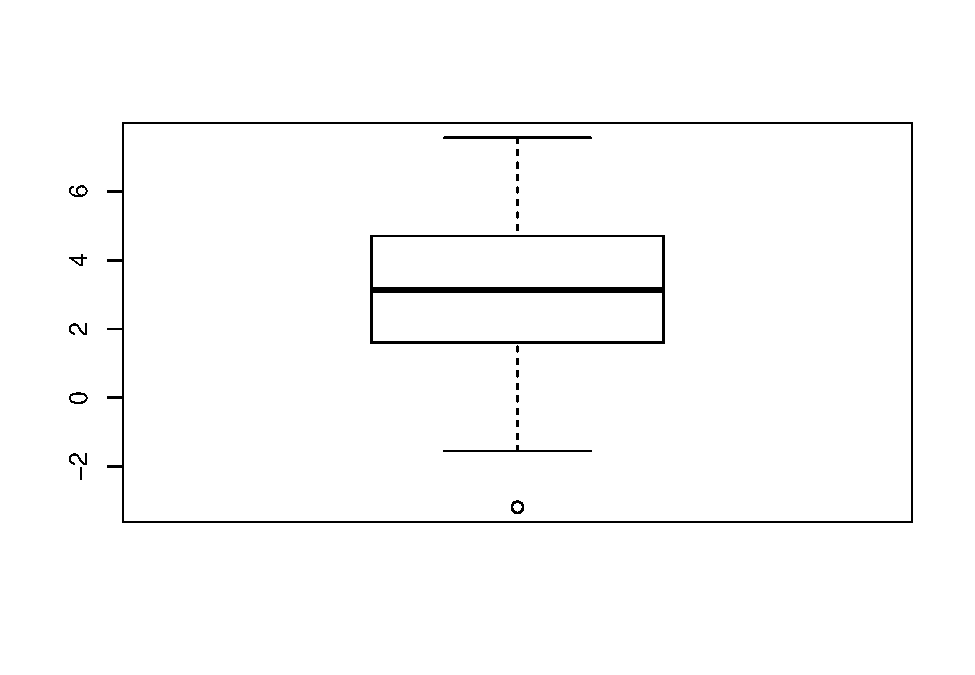
\includegraphics{wtloss_notebook_files/figure-latex/unnamed-chunk-6-1.pdf}

\subsection{Via ggplot2's ggplot
function}\label{via-ggplot2s-ggplot-function}

\begin{Shaded}
\begin{Highlighting}[]
\KeywordTok{ggplot}\NormalTok{(wtloss, }\KeywordTok{aes}\NormalTok{(}\DataTypeTok{y =}\NormalTok{ lbslost)) }\OperatorTok{+}
\StringTok{  }\KeywordTok{geom_boxplot}\NormalTok{()}
\end{Highlighting}
\end{Shaded}

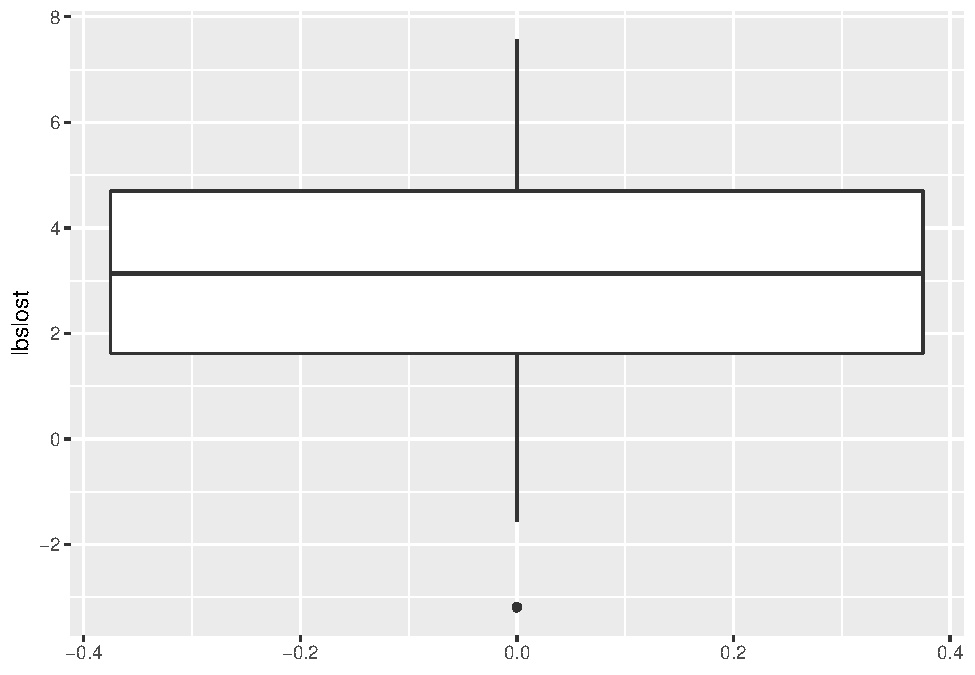
\includegraphics{wtloss_notebook_files/figure-latex/unnamed-chunk-7-1.pdf}

The boxplot indicates that there is one outlier for lbslost, with a
value of -4. This indicates that one participant gained 4 pounds during
the course of this study.

\section{Plot relationships between
variables}\label{plot-relationships-between-variables}

\subsection{Via Base R's plot function}\label{via-base-rs-plot-function}

\begin{Shaded}
\begin{Highlighting}[]
\KeywordTok{attach}\NormalTok{(wtloss)}
\KeywordTok{plot}\NormalTok{(lbslost, caldef )}
\end{Highlighting}
\end{Shaded}

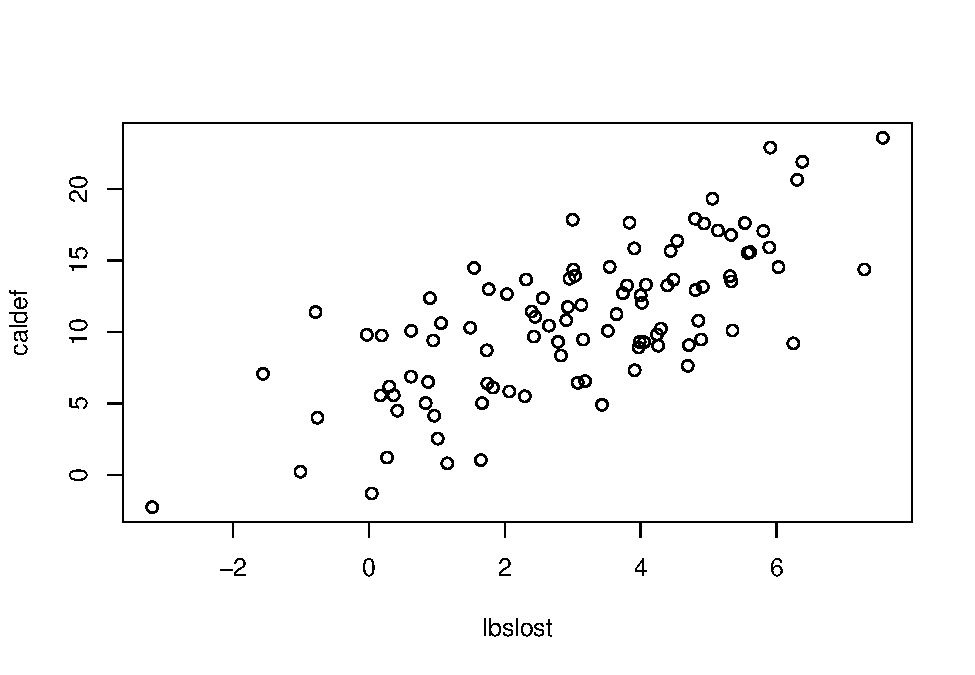
\includegraphics{wtloss_notebook_files/figure-latex/unnamed-chunk-8-1.pdf}

\begin{Shaded}
\begin{Highlighting}[]
\KeywordTok{plot}\NormalTok{(lbslost, selfeff)}
\end{Highlighting}
\end{Shaded}

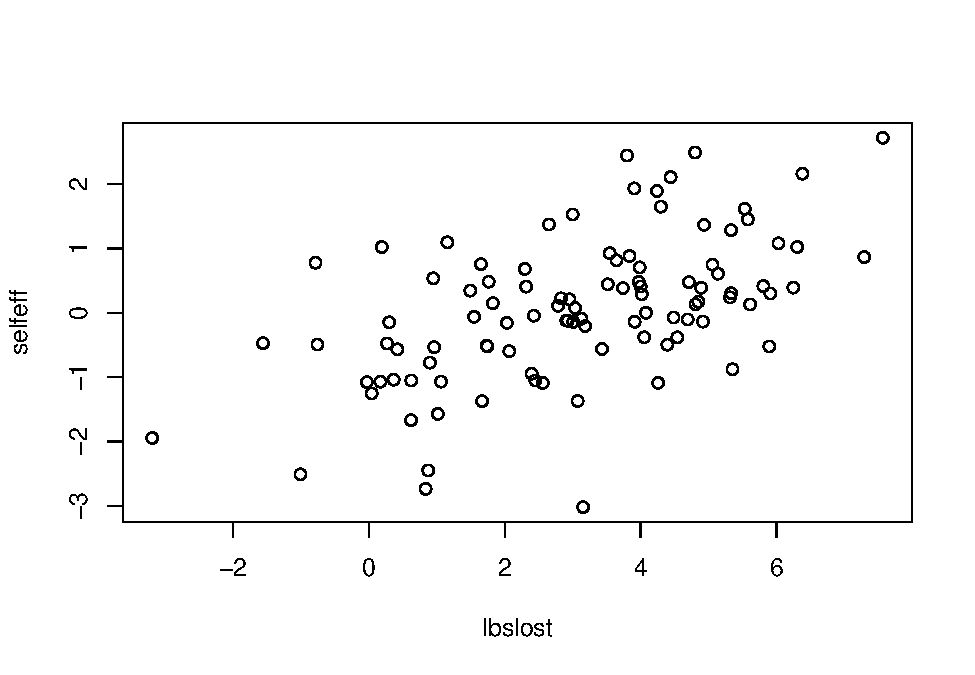
\includegraphics{wtloss_notebook_files/figure-latex/unnamed-chunk-8-2.pdf}

\begin{Shaded}
\begin{Highlighting}[]
\KeywordTok{plot}\NormalTok{(caldef , selfeff)}
\end{Highlighting}
\end{Shaded}

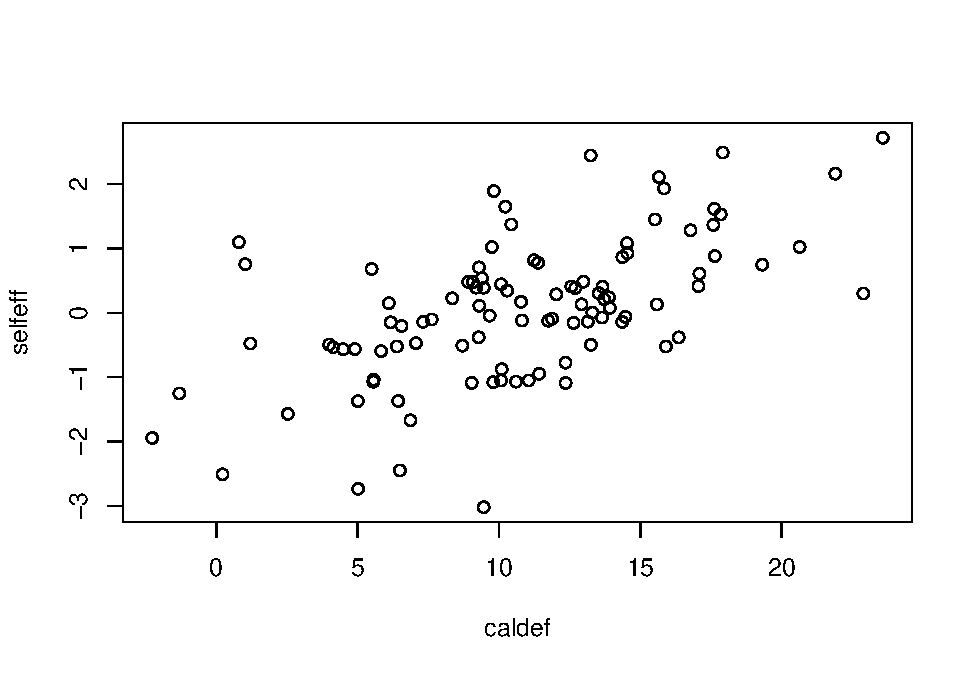
\includegraphics{wtloss_notebook_files/figure-latex/unnamed-chunk-8-3.pdf}

\begin{Shaded}
\begin{Highlighting}[]
\KeywordTok{detach}\NormalTok{(wtloss)}
\end{Highlighting}
\end{Shaded}

\subsection{Via ggplot2's ggplot
function}\label{via-ggplot2s-ggplot-function-1}

\begin{Shaded}
\begin{Highlighting}[]
\KeywordTok{ggplot}\NormalTok{(wtloss, }\KeywordTok{aes}\NormalTok{(}\DataTypeTok{x =}\NormalTok{ caldef, }\DataTypeTok{y =}\NormalTok{ lbslost)) }\OperatorTok{+}
\StringTok{  }\KeywordTok{geom_point}\NormalTok{() }\OperatorTok{+}
\StringTok{  }\KeywordTok{geom_smooth}\NormalTok{(}\DataTypeTok{method =} \StringTok{"lm"}\NormalTok{)}
\end{Highlighting}
\end{Shaded}

\begin{verbatim}
## `geom_smooth()` using formula 'y ~ x'
\end{verbatim}

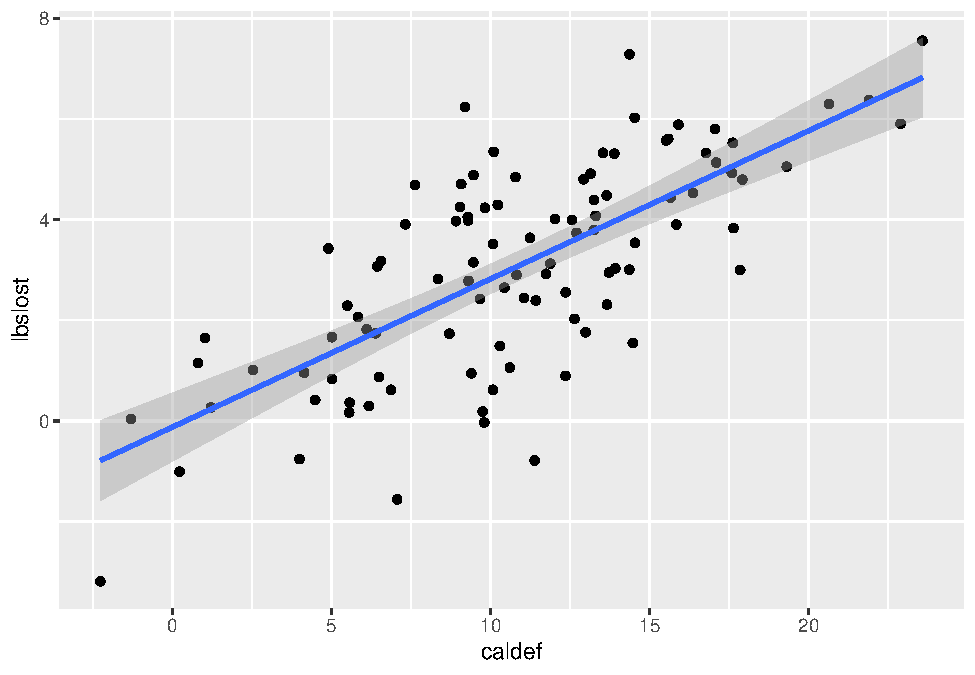
\includegraphics{wtloss_notebook_files/figure-latex/unnamed-chunk-9-1.pdf}

\begin{Shaded}
\begin{Highlighting}[]
\KeywordTok{ggplot}\NormalTok{(wtloss, }\KeywordTok{aes}\NormalTok{(}\DataTypeTok{x =}\NormalTok{ lbslost, }\DataTypeTok{y =}\NormalTok{ selfeff)) }\OperatorTok{+}
\StringTok{  }\KeywordTok{geom_point}\NormalTok{() }\OperatorTok{+}
\StringTok{  }\KeywordTok{geom_smooth}\NormalTok{(}\DataTypeTok{method =} \StringTok{"lm"}\NormalTok{)}
\end{Highlighting}
\end{Shaded}

\begin{verbatim}
## `geom_smooth()` using formula 'y ~ x'
\end{verbatim}

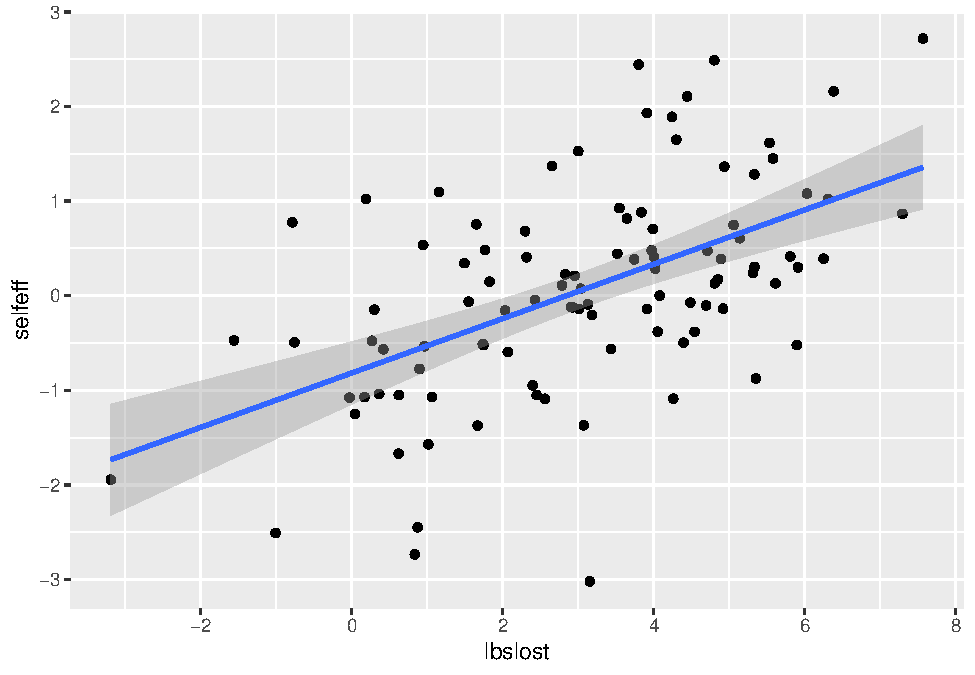
\includegraphics{wtloss_notebook_files/figure-latex/unnamed-chunk-9-2.pdf}

\begin{Shaded}
\begin{Highlighting}[]
\KeywordTok{ggplot}\NormalTok{(wtloss, }\KeywordTok{aes}\NormalTok{(}\DataTypeTok{x =}\NormalTok{ caldef, }\DataTypeTok{y =}\NormalTok{ selfeff)) }\OperatorTok{+}
\StringTok{  }\KeywordTok{geom_point}\NormalTok{() }\OperatorTok{+}
\StringTok{  }\KeywordTok{geom_smooth}\NormalTok{(}\DataTypeTok{method =} \StringTok{"lm"}\NormalTok{)}
\end{Highlighting}
\end{Shaded}

\begin{verbatim}
## `geom_smooth()` using formula 'y ~ x'
\end{verbatim}

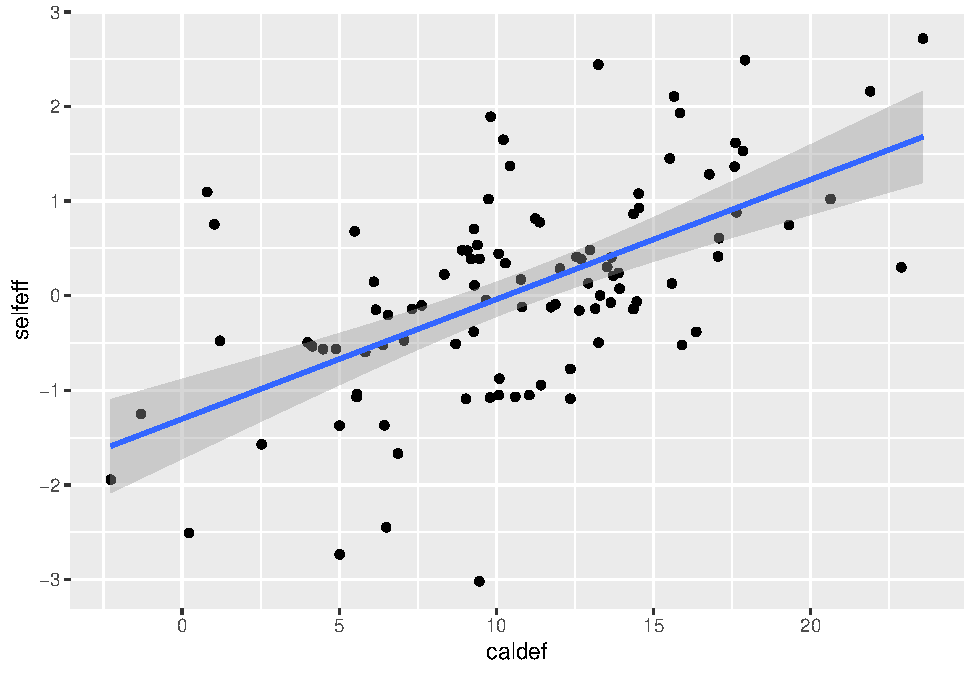
\includegraphics{wtloss_notebook_files/figure-latex/unnamed-chunk-9-3.pdf}

\section{Correlations}\label{correlations}

\subsection{Pearson's Correlations
Matrices}\label{pearsons-correlations-matrices}

\subsubsection{Via Base R's cor
function}\label{via-base-rs-cor-function}

\begin{Shaded}
\begin{Highlighting}[]
\KeywordTok{cor}\NormalTok{(wtloss)}
\end{Highlighting}
\end{Shaded}

\begin{verbatim}
##                  id    lbslost      caldef     selfeff
## id       1.00000000 -0.1425016 -0.07237732 -0.05700845
## lbslost -0.14250157  1.0000000  0.72174587  0.54278360
## caldef  -0.07237732  0.7217459  1.00000000  0.58508654
## selfeff -0.05700845  0.5427836  0.58508654  1.00000000
\end{verbatim}

\subsubsection{Via apaTables' apa.cor.table
function}\label{via-apatables-apa.cor.table-function}

\begin{Shaded}
\begin{Highlighting}[]
\KeywordTok{apa.cor.table}\NormalTok{(wtloss, }\StringTok{"wtloss correlations.doc"}\NormalTok{, }\DataTypeTok{show.conf.interval =} \OtherTok{TRUE}\NormalTok{)}
\end{Highlighting}
\end{Shaded}

\begin{verbatim}
## 
## 
## Means, standard deviations, and correlations with confidence intervals
##  
## 
##   Variable   M     SD    1           2          3         
##   1. id      50.50 29.01                                  
##                                                           
##   2. lbslost 3.06  2.10  -.14                             
##                          [-.33, .06]                      
##                                                           
##   3. caldef  10.80 5.14  -.07        .72**                
##                          [-.27, .13] [.61, .80]           
##                                                           
##   4. selfeff 0.06  1.11  -.06        .54**      .59**     
##                          [-.25, .14] [.39, .67] [.44, .70]
##                                                           
## 
## Note. M and SD are used to represent mean and standard deviation, respectively.
## Values in square brackets indicate the 95% confidence interval.
## The confidence interval is a plausible range of population correlations 
## that could have caused the sample correlation (Cumming, 2014).
## * indicates p < .05. ** indicates p < .01.
## 
\end{verbatim}

Correlation coefficients measure the direction and strength of the
tendnecy for two variables to vary together. Correlation coefficients do
not apply causation.

The correlation coefficient between lbslos and caldef is .72, and this
is significant at p\textless{}0.01. Thus, there is a strong, positive
(uphill) correlation between lbslost and caldef.

The correlation coefficient between lbslost and selfeff is .54, and this
is significant at p\textless{}0.01. Thus, there is a strong, positive
(uphill) correlation between lbslost and selfeff.

The correlation between caldef and selfeff is .59, and this is
significant at p\textless{}0.01. Thus, there is a strong, positive
(uphill) correlation between caldef and selfeff.

The correlation between lbslost and caldef is larger than the
correlations between lbslost and selfeff and between caldef and selfeff.

\subsection{Get partial correlation}\label{get-partial-correlation}

\begin{Shaded}
\begin{Highlighting}[]
\KeywordTok{attach}\NormalTok{(wtloss)}
\KeywordTok{pcor.test}\NormalTok{(lbslost, caldef, selfeff)}
\end{Highlighting}
\end{Shaded}

\begin{verbatim}
##    estimate      p.value statistic   n gp  Method
## 1 0.5933978 9.634079e-11  7.260806 100  1 pearson
\end{verbatim}

\begin{Shaded}
\begin{Highlighting}[]
\KeywordTok{detach}\NormalTok{(wtloss)}
\end{Highlighting}
\end{Shaded}

Partial correlation first removes from both the outcome (lbslost) and
predictor (caldef) all variance which may be accounted for by a third
variable (in this case selfeff). Then it correlates the remaining
variance of caldef with the remaining variance of lbslost. Here, the
partial correlation between lbslost and caldef is .593 and this is
significant at p\textless{}0.01. Thus, there is still a strong, positive
(uphill) correlation between lbslost and caldef when controlling for or
holding constant the effects of selfeff. This correlation is smaller
than when the effects of selfeff were not removed (.593 compared to
0.722).

\subsection{Get semipartial
correlation}\label{get-semipartial-correlation}

\begin{Shaded}
\begin{Highlighting}[]
\KeywordTok{attach}\NormalTok{(wtloss)}
\KeywordTok{spcor.test}\NormalTok{(lbslost, caldef, selfeff)}
\end{Highlighting}
\end{Shaded}

\begin{verbatim}
##    estimate      p.value statistic   n gp  Method
## 1 0.4983786 1.525307e-07  5.661694 100  1 pearson
\end{verbatim}

\begin{Shaded}
\begin{Highlighting}[]
\KeywordTok{detach}\NormalTok{(wtloss)}
\end{Highlighting}
\end{Shaded}

Semi-partial correlation first removes from the predictor (caldef) all
variance which may be accounted for by the other predictors (in this
case selfeff). Then it correlates the remaining variance of the
predictor (caldef) with y (lbslost). Here the semi-partial correlation
between caldef and lbslost is .498, and this is significant at
p\textless{}0.01. Thus, there is still a positive (uphill) relationship
between lbs and caldef, but this correlation is smaller (now moderately
strong; 0.498 compared to 0.722) than when the effects of selfeff on
caldef were not controlled for.

Note: the semi-partial correlation is often considered to be a better
indicator of the ``actual relevance'' of a predictor, because it is
scaled relative the total variability of the outcome variable. The
squared semi-partial correlation will give you the proportion of unique
variance accounted for by the predictor, relative to the total variance
of Y. This is a key concept in Multiple Linear Regression models.

\section{Fit a Simple Linear Regression (SLR)
Model}\label{fit-a-simple-linear-regression-slr-model}

\begin{Shaded}
\begin{Highlighting}[]
\NormalTok{mod1 <-}\StringTok{ }\KeywordTok{lm}\NormalTok{(lbslost }\OperatorTok{~}\StringTok{ }\NormalTok{caldef, }\DataTypeTok{data =}\NormalTok{ wtloss)}
\end{Highlighting}
\end{Shaded}

\subsection{Display SLR model results}\label{display-slr-model-results}

\subsubsection{Via base R's summary
function}\label{via-base-rs-summary-function-1}

\begin{Shaded}
\begin{Highlighting}[]
\KeywordTok{summary}\NormalTok{(mod1)}
\end{Highlighting}
\end{Shaded}

\begin{verbatim}
## 
## Call:
## lm(formula = lbslost ~ caldef, data = wtloss)
## 
## Residuals:
##     Min      1Q  Median      3Q     Max 
## -4.0197 -0.9480  0.0838  1.1227  3.6602 
## 
## Coefficients:
##             Estimate Std. Error t value Pr(>|t|)    
## (Intercept) -0.12079    0.34127  -0.354    0.724    
## caldef       0.29473    0.02855  10.323   <2e-16 ***
## ---
## Signif. codes:  0 '***' 0.001 '**' 0.01 '*' 0.05 '.' 0.1 ' ' 1
## 
## Residual standard error: 1.46 on 98 degrees of freedom
## Multiple R-squared:  0.5209, Adjusted R-squared:  0.516 
## F-statistic: 106.6 on 1 and 98 DF,  p-value: < 2.2e-16
\end{verbatim}

\subsubsection{Via olsrr's ols\_regress
function}\label{via-olsrrs-ols_regress-function}

\begin{Shaded}
\begin{Highlighting}[]
\KeywordTok{ols_regress}\NormalTok{(mod1)}
\end{Highlighting}
\end{Shaded}

\begin{verbatim}
##                         Model Summary                          
## --------------------------------------------------------------
## R                       0.722       RMSE                1.460 
## R-Squared               0.521       Coef. Var          47.647 
## Adj. R-Squared          0.516       MSE                 2.131 
## Pred R-Squared          0.504       MAE                 1.149 
## --------------------------------------------------------------
##  RMSE: Root Mean Square Error 
##  MSE: Mean Square Error 
##  MAE: Mean Absolute Error 
## 
##                                ANOVA                                 
## --------------------------------------------------------------------
##                Sum of                                               
##               Squares        DF    Mean Square       F         Sig. 
## --------------------------------------------------------------------
## Regression    227.034         1        227.034    106.558    0.0000 
## Residual      208.801        98          2.131                      
## Total         435.835        99                                     
## --------------------------------------------------------------------
## 
##                                   Parameter Estimates                                   
## ---------------------------------------------------------------------------------------
##       model      Beta    Std. Error    Std. Beta      t        Sig      lower    upper 
## ---------------------------------------------------------------------------------------
## (Intercept)    -0.121         0.341                 -0.354    0.724    -0.798    0.556 
##      caldef     0.295         0.029        0.722    10.323    0.000     0.238    0.351 
## ---------------------------------------------------------------------------------------
\end{verbatim}

The intercept represents the value of y when x = 0. Here, the intercept
for caldef is -0.121, indicating that lbslost = -0.121 when caldef = 0.

The beta for a predictor represents the expected change in y for a
1-unit increase in x. Here, the beta for caldef is 0.295, indicating
that lbslost is expected to increase by 0.295 for every 1-unit increase
in caldef. The standard error for this estimate is 0.029, indicating
that the average distance that the observed values fall from the
predicted regression line is 0.029. The upper and lower confidence
intervals for this value indicate that there is a 95\% liklihood that
the true value for this beta estimate falls between 0.238 and 0.351.
Because the 95\% confidence interval for the estimate does not include
zero, and becuase p \textless{} .001, this effect is significant.

The model R\^{}2 value represents the proportion of variability in y
that the model explains. Here, the model R\^{}2 is 0.521, indicating
that the predictor (caldef) explains 52.1\% of the variability in
lbslost.

\end{document}
